\section{Theorie}
\label{sec:Theorie}

Damit ein Atomkern stabil sein kann, darf das Verhältnis zwischen der Anzahl an Neutronen und Protonen nur in einem 
kleinen Intervall variieren. Instabile Atomkerne zerfallen nach einer gewissen Zeit, die je nach Atom unterschiedlich ist.
Die sogenannte Halbwertszeit $T$ gibt aussage über die Zerfallswahrscheinlichkeit eines bestimmten Atoms, indem diese angibt,
nach welcher Zeit bei hinreichend großer Anzahl an gleichartigen Kernen die Hälfte dieser zerfallen ist. Über die Gleichung 
\begin{equation}
    N(t) = N_0 e^{-\lambda t}
    \label{eqn:nt}
\end{equation}
kann die Anzahl der zum Zeitpunkt $t$ noch bestehenden Kerne $N(t)$ beschrieben werden. Dabei ist $N_0$ die Anzahl der zum 
Zeitpunkt $t=0$ vorhandenen Kerne und $\lambda$ die Zerfallskonstante, die je nach Isotop variiert. Nach der bereits geannten 
Halbwertszeit $T$ ergibt sich dann die Gleichung zu 
\begin{equation}
    \frac{1}{2}N_0 = N_0 e^{-\lambda T}\,,
\end{equation}
wodurch sich die Halbwertszeit in Abhängigkeit der Zerfallskonstante $\lambda$ durch 
\begin{equation}
    T = \log{\frac{2}{\lambda}}
\end{equation}
beschreiben lässt.
\\
Die Halbwertszeiten unterschiedlicher Elemente variieren dabei jedoch über $23$ $10$-er Potenzen, was unterschiedliche 
Messverfahren je nach Größenordung von $T$ erfordert. Daher wird im vorliegenden Versuch die Untersuchung auf Elemente, deren 
Halbwertszeiten in der Größenordung Sekunden bis Stunden liegt, beschränkt. Um bei derartigen Elementen möglichst genaue Messungen
durchzuführen, müssen die Atomkerne kurz vor der Messung erzeugt werden. Dazu werden stabile Atome mit Neutronen beschossen, 
wodurch diese mit einem veränderten Verhältnis an Protonen und Neutronen in einen instabilen Zustand übergehen und letztendlich
zerfallen. Um die Wahrscheinlichkeit möglichst hoch zu halten, dass ein Neutron vom Kern eingefangen wird, sollte die kinetsiche
Energie des Neutrons und damit auch seine Geschwindigkeit gering gehalten werden. Der Wirkungsquerschnitt $\sigma$ ist dabei ein
Maß für die Wahrscheinlichkeit einer Kernreaktion bei einem eintreffenden Neutron. Die Abhängigkeit von der Energie lässt sich 
über 
\begin{equation}
    \sigma \propto \frac{1}{\sqrt{E}}
\end{equation}
darstellen.
Damit ein Neutron beim auftreffen auf den Atomkern eine hinreichend geringe Energie aufweist, muss dieses vorher abgebremst werden.
Die dafür erforderliche Vorgehensweise wird im Abschnitt \ref{sec:Durchführung} beschrieben.
\\
Es ist problematisch, das in Gleichung \ref{eqn:nt} genannte $N(t)$ zu bestimmen. Deutlich einfacher lässt sich die Anzahl 
$N_{\Delta t}(t)$ der in einem bestimmen Zeitraum zerfallenden Kerne ermitteln. Über die Gleichung 
\begin{equation}
    \log{N_{\Delta t}(t)} = \log{N_0}(1 - e^{-\lambda\Delta t}) -\lambda t
\end{equation}
lässt sich dann mit einer linearen Ausgleichsrechung die Zerfallskonstante $\lambda$ bestimmen, die auf die Halbwertszeit
zurückzuführen ist. Dabei sollte auf ein geeignetes Zeitintervall $\Delta t$ geachtet werden, da es sonst zu großen systematischen
oder statistischen Fehlern kommen kann. 
\\
Einige Elemente weisen die Eigenschaft auf, bei der Aktivierung mit Neutronen auf zwei verschiedene Weisen zu zerfallen. Ein 
Beispiel dafür ist das natürliche Silber, welches aus zwei unterschiedlichen Isotopen besteht. Diese haben jeweils verschiedene
Zerfallskonstanten und so auch verschiedene Halbwertszeiten. In der Abbildung \ref{fig:2iso} ist die Zerfallskurve von zwei
sich überlagernden Zerfällen zweier Isotope zu sehen 
\begin{figure}
    \centering
    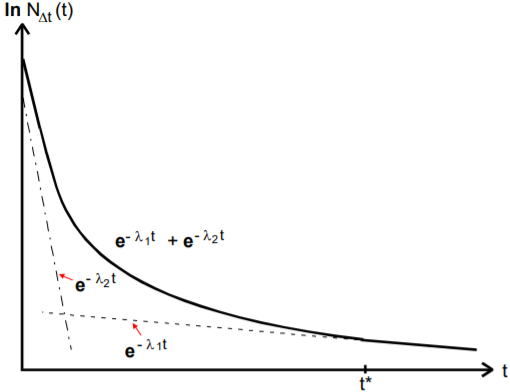
\includegraphics[width=\textwidth]{data/zerfall.png}
    \caption{Zerfall zweier Isotope mit unterschiedlichen Zerfallskonstanten}
    \label{fig:2iso}
\end{figure}
Zur Bestimmung der Halbwertszeit wird zuerst die des langsam zerfallenden Isotops untersucht. Dafür werden nur Messwerte nach dem 
Zeitpunkt $t*$ betrachtet. Mit diesen Werten wird eine lineare Ausgleichsrechung durchgeführt, wodurch dann die Zerfallskonstante
des langlebigen Isotops bestimmt werden kann. Die so berechneten Werte $N_\text{lang}(t)$ können dann von den Messwerten 
subtrahiert werden und es kann eine weitere Ausgleichsrechung durchgeführt werden, um die Zerfallskonstante des kurzlebigen
Isotops zu bestimmen. 